\def\year{2019}\relax
%File: formatting-instruction.tex
\documentclass[letterpaper]{article} %DO NOT CHANGE THIS
\usepackage{aaai19}  %Required
\usepackage{times}  %Required
\usepackage{helvet}  %Required
\usepackage{courier}  %Required
\usepackage{url}  %Required
\usepackage{graphicx}  %Required
\usepackage{subcaption}
\usepackage{amsmath}
\usepackage{graphics}

\frenchspacing  %Required
\setlength{\pdfpagewidth}{8.5in}  %Required
\setlength{\pdfpageheight}{11in}  %Required
%PDF Info Is Required:
  \pdfinfo{
/Title (The XAI Paradox: Systems that Perform Well for the Wrong Reasons)
/Author (Cor Steging, Lambert Schomaker, Bart Verheij)}
\setcounter{secnumdepth}{0}  
 \begin{document}
% The file aaai.sty is the style file for AAAI Press 
% proceedings, working notes, and technical reports.
%
\title{The XAI Paradox: Systems that Perform Well for the Wrong Reasons}
\author{Cor Steging, Lambert Schomaker, Bart Verheij\\
Department of Artificial Intelligence, Bernoulli Institute\\
University of Groningen\\
}
\maketitle
\begin{abstract}
Many of the successful modern machine learning approaches can be described as ``black box'' systems; these systems perform well, but are unable to explain the reasoning behind their decisions. The emerging sub-field of Explainable Artificial Intelligence (XAI) aims to create systems that are able to explain to their users why they made a particular decision. Using artificial datasets whose internal structure is known beforehand, this study shows that the reasoning of systems that perform well is not necessarily sound. Furthermore, when multiple combined conditions define a dataset, systems can perform well on the combined problem and not learn each of the individual conditions. Instead, a confounding structure within the data is learnt that still allows making the correct decisions. With regards to the goal of creating explainable systems, however, unsound rationales could create irrational explanations which would be problematic for the XAI movement.
\end{abstract}

\section{Introduction}
In recent years, the notion of artificial intelligence has reached the masses with the introduction of smart devices, digital assistants, self-driving cars and many other inventions. This booming interest in AI can largely be attributed to the success of machine learning in combination with the growing availability of big data. Despite their success, many of the most commonly employed machine learning techniques inherently lack a possibility to provide an explanation of the way in which they reason. These ``black box'' systems are often distrusted by their users because they do not explain why particular decisions are made (cf. also the discussion about a `right to an explanation' in the EU General Data Protection Act; see e.g. \cite{edwards2017slave}).

The response to the lack of transparency is the emerging field of Explainable Artificial Intelligence (XAI) \cite{gunning2017explainable}. XAI aims to create explainable models that are able to explicitly describe the inner workings of a ``black box'' machine learning system, and thus provide the essential explanations to their users. Examples of such XAI systems are rule extraction algorithms, such as \cite{lu2017neurorule}, that create  sets of rules for the users that describe the reasoning of ``black box'' systems, or glass-box systems, like \cite{holzinger2017glass}, in which the users are able to influence what the systems learn. Yet another approach is used in a recent deep learning system for diagnosing retinal diseases (outperforming medical experts). The system is divided into a framework of smaller systems; one for each stage of the diagnostic process \cite{de2018clinically}, making it easier for the clinicians to investigate and understand the reasoning of the system. In these and different ways, XAI systems aim to yield accurate and meaningful explanations of their reasoning, without sacrificing performance. 

A question that must be asked in XAI research is whether or not the explanation that a XAI system gives indeed makes sense in the domain. That this is not a trivial issue is in particular suggested by the phenomenon of adversarial examples in image classification, where input images are slightly altered using a perturbation \cite{yuan2017adversarial}. To the human eye, there is no apparent difference between the original input image and its altered version, while a machine learning system makes a completely different classification after the image is altered. This suggests that the understanding that the systems have differs strongly from that of humans, despite the fact that the system usually makes the correct classifications. In other words, systems perform well, but apparently for the wrong reasons. In and of itself, this is still impressive, as the machine learning system is able to extrapolate structures from the data that we as humans are not able to perceive, and consequently achieve a high performance. As a result, however, we can expect that when an explainable model is generated from these systems using XAI techniques, explanations that are generated may not make sense to the users, countering the desired transparancy and decreasing trust. 

The aim of this study is to investigate this question: to what extent do systems learn structures that make sense in a domain? In order to operationalize this idea, we generate structured datasets, where the embedded structure is a model of what makes sense in a domain. We investigate machine learning techniques in terms of how well they are able to learn the structure that defines datasets, rather than only in terms of a general performance accuracy. More specifically, artificial datasets will be generated from a set of predetermined formal conditions in terms of symmetric Boolean functions, on which machine learning systems will train. In this way, we can study how well the systems are able to extrapolate the correct conditions from the data. By combining multiple conditions defining datasets, we can investigate interaction effects whether the system learns each of the individual conditions correctly, or instead learns a different confounding structure that still accurately maps the input to the output. 

Our method of using artificial datasets with predetermined structure was inspired by neural network research in a legal setting \cite{bench1993neural}, a 1990s study of XAI themes in the field of AI \& Law. In that field, XAI issues arose already then, since explainability and transparency are especially pertinent in the law, where decisions must be made for the right reasons. That work used a specific legal example. We present an abstract, parameterized set of problems (defined using families of symmetric Boolean functions) in order to gain more insights about the task of learning structure that makes sense in a domain. Before describing our specific method and results, we discuss the findings of \cite{bench1993neural}.

\section{Previous Research:  \\the Welfare Benefit Dataset}
\cite{bench1993neural} uses a particular case study in the field of law investigating whether neural networks can achieve a high performance on open texture law problems. In that work, it is examined whether or not the rationale that the neural networks use in their classification is acceptable. To this end, a fictional dataset is generated that describes the personal information of elderly people and whether they are eligible for a particular welfare benefit. The eligibility depends on the six conditions shown below, and the personal information of the individual. If and only if all of the six conditions apply to an individual, her or she is eligible for a benefit. 

\begin{enumerate}
\item
The person should be of pensionable age (60 for a woman, 65 for a man).
\item
The person should have paid contributions in four out of the last five relevant contribution years. 
\item
The person should be a spouse of the patient.
\item
The person should not be absent from the UK.
\item
The person should have capital resources not amounting to more than \pounds 3,000.
\item 
If the relative is an in-patient the hospital should be within a certain distance: if an out-patient, beyond that distance.
\end{enumerate}

\noindent Neural networks are trained on this dataset and tasked with predicting the eligibility of new individuals. High classification accuracies are achieved by these neural networks, with the number of correct predictions ranging from 98.75\% to 99.25\%. 

In order to determine how well the conditions that define eligibility are learned by networks, special test datasets are generated for each condition, in which the personal information is generated such that all other conditions are satisfied. For instance, the first condition states that the person should be of pensionable age, which is 60 for women and 65 for men. In order to measure how well this condition is learned by a network, a test dataset is generated with values for the age and gender variables across the full possible range of values. The values of the remaining variables are generated such that they satisfy the other five conditions. In this way, a high performance on the resulting test dataset can only be achieved if the network has learned the condition 'the person should be of pensionable age'.

The research shows that the networks are unable to learn all of the conditions that define eligibility, despite the high classification accuracy. The condition of pensionable age, for instance, is not learned correctly by the networks. Bench-Capon shows that a high classification accuracy can be obtained in this example by only having learned a few of the conditions. By altering the statistical distribution of the training dataset it was possible to improve upon how well certain conditions are learned, but accurately learning all of them was not achieved. The actual conditions and structures that define this dataset are therefore not learned by the networks. In this particular example, a high performance does therefore not necessarily guarantee a sound rationale.

In followup research, a comparison was made between the performance of the neural networks \cite{bench1993neural},  defeasible logic \cite{johnston2003induction} and an adaptation of the CN2 algorithm using argumentation \cite{movzina2005argument} on the the same fictional welfare benefit dataset. All systems produced a high classification accuracy, but none of them were able to exactly reproduce all of the six conditions of the dataset. Additionally, it was shown that conditions 3 and 4, the simple boolean conditions, are easily identified by all of the systems. Similarly, the systems seem to have no difficulty in identifying condition 5, in which a specific threshold value needs to be exceeded. Conditions 1 and 6 on the other hand, in which specific combinations of two variables are required, are difficult for the systems to learn.  Additionally, so-called condition 2, in which at least 4 out of the 5 variables need to be true, are not easily identified by the system either. 

This research showed that for the welfare benefit dataset good performance could be achieved without completely learning the structure embedded in the data. In the present study we aim to gain more insight in this phenomenon. For this, we construct a series of structured data sets in terms of symmetric Boolean functions.

\section{Method: Symmetric Boolean Functions}
We saw that in the welfare benefit dataset the systems were unable to learn all of the conditions that defined the data, despite achieving a high classification accuracy. Individually, the conditions were quite simple and all modern machine learning systems should be able learn them. Combined, however, they become more difficult to learn. This could indicate that there might be a type of interaction effect between conditions, that causes a condition to be learned less successfully when other conditions are present. For instance, a machine learning algorithm may be able to easily learn two conditions separately, but have difficulty when attempting to learn both at the same time. This study sets out to investigate how well machine learning systems are able to internalize such conditions that define a training dataset. Furthermore, the possible interaction effect between conditions will be examined.

We use %The type of functions that neural networks and other machine learning algorithms have been shown to struggle with in previous research can be generalized into 
symmetrical Boolean functions. The output of these functions is only based on the number of 1's in the input vector, hence the location of the 1's in the input vector is irrelevant. An example of a symmetrical Boolean function with two variables is the XOR function (well-known for its role in the history of neural networks), which provides an output of 1 if and only if the number of 1's in the input vector is equal to 1. With more than two variables, the XOR function can be generalized to the parity function, which is a function that returns an output of 1 if and only if there is an odd number of 1's in the input vector. We use three families of symmetrical Boolean functions \cite{wegener1987complexity}:

\begin{itemize}
\item
Parity function:  $f^n(x) = 1 \leftrightarrow |x| \equiv 1 \text{ mod } 2$. 
\item
Exact value function:  $f^n_m(x) = 1 \leftrightarrow |x|= m$.
\item
M-out-of-N function: $f^n_m(x) = 1 \leftrightarrow |x| \geq m$. 
\end{itemize}

\noindent Here $|x|$ denotes the number of 1's in vector $x$. All functions have integer parameter $n$ for the length of the Boolean input vector $x$ with $n$ values. The exact value and M-out-of-N functions have an additional integer parameter $m \leq n$. These three families of symmetrical Boolean functions form the basis of the conditions that define datasets as they are used in our experiments. 

\subsection{Datasets}
%%%BV VERHELDEREN
For our experiment, a parameterized series of datasets is generated based on conditions defined in terms of symmetrical Boolean functions. Each instance in the dataset has an output value, which is true if and only if all of its conditions are true as well. This set of conditions can include the M-out-of-N function, the exact value function and the parity function. Each condition also has a set of parameters. As described earlier, parameter $n$ denotes the number of variables of the condition and parameter $m$ is used in M-out-of-N functions and exact value functions to determine the value of the output. The total number of variables of each instances in the datasets is therefore based on the number of variables of each of the conditions.

For any set of conditions, the following datasets are generated: a training set, a general test set and a specific test set for each condition. First of all, a training set consists of 150,000 instances where half of the instances are generated randomly such that their output value is true, and the other half are generated randomly such that their output value is false.  In the latter half, the instances are generated such that they fail on each of its conditions equally. With two conditions for example, this means that the latter half (the half where the output is false) would consists for 50\% out of instances where the first condition is false and for 50\% out of instances where the second condition is false. If a condition is not specifically set up to fail, its variables are provided with random values. The general test set consists of 150,000 instances, and is generated in the exact same fashion.

For each condition, an additional specific test set is generated. This test set is used to determine how well a system is able learn a specific condition. Given such a condition, its test set is constructed by generating all of the possible input values that the condition can have. For example, the XOR condition (or parity function with $n$=2) has $2^2=4$ possible values and would therefore have a specific test set with 4 instances. The variables of any additional conditions are given random values such that these conditions are satisfied. This ensures that the output is dependent on only the single condition for which the test set is generated. This allows us to measure how well that particular condition is learned by the system. 



\subsection{Machine Learning Algorithms}
Both a decision tree algorithm and a neural network are trained on the training sets. The resulting systems are tasked with classifying the general test sets and the specific test sets. The decision tree system uses the CART algorithm %%%BV REFERENCE INVOEGEN
with the Gini impurity and it does not make use of early stopping or any other form of pruning. The neural networks used consist of three hidden layers, with 25, 10 and 3 hidden nodes respectively. The learning rate is set to 0.05 and the sigmoid is used as the activation function. The networks use a mini-batch approach with a batch size of 50. The maximum number of times that the entire training dataset will be presented to the network during the training phase is set to 2000 rounds. Training stops early if there is no change in training errors over the past 10 rounds.

%%%BV INCLUDE A SUBSECTION `Experiments' HERE where you describe all experiments, including noise

\section{Results}
%%%BV REDUCE DISCUSSION IN THIS SECTION, MOVE TO DISCUSSION SECTION IF POSSIBLE

Both machine learning systems are first trained and tested using datasets with only a single condition; either the parity, M-out-of-N or exact value function. This will determine whether the systems are able to learn each of the conditions individually. The systems will then be trained and tested on datasets with two conditions in order to investigate both how well the systems are able to learn the combined problem and how well they are able to learn the individual conditions that make up the combined problem.

\subsection{Single Condition Datasets}
First of all, datasets are generated with only one condition with different numbers of variables $n$; from 2 to 18.  For the M-out-of-N and exact value condition, the value of $m$ will be varied as well: between 1 and $n$. For each condition and each possible combination of $m$ and $n$, both the decision tree algorithm and the neural network are trained on the training dataset and then tested on the general test set and the specific condition test set. In Figure \ref{fig:DTvsNN} the accuracy of the decision tree and the neural network on the general test set is shown versus the number of variables for all three conditions. For the M-out-of-N and exact value condition, the mean accuracies across all possible values values of $m$ are displayed.

The accuracies of these systems on the specific test sets were almost identical, and a repeated measures anova showed no significant difference between the performance on the general test set and on the specific test set for all of the conditions. Figure \ref{fig:DTvsNN} shows that the accuracy of the decision tree system starts to decrease as the number of variables of the condition increases. The neural network does not appear to have difficulties with any of the conditions, as the mean accuracy for each number of variables never reaches lower than 98\%. Earlier research has shown that with sufficient training and enough hidden nodes, a neural network should theoretically be able to learn any parity function \cite{wilamowski2003solving}. If we assume that a similar rule applies to the other types of symmetrical Boolean functions, the 150,000 training instances appear to be sufficient for a network of this format to learn the conditions. Clearly, this is not sufficient for the decision tree algorithm for higher values of variables. The average accuracy of the neural network is relatively stable near 100\% for each condition and each number of variables. The accuracy of the decision tree decreases at around 14 variables for all three conditions. The accuracy on the parity condition drops rapidly to 55\% with 18 variables, whereas the accuracies of the exact value and M-out-of-N conditions decrease to 89\% and 96\% respectively at 18 variables. 

%%%BV TURN INTO SVGs/PDFs
%%%BV INCREASE FONT SIZES

 \begin{figure}[h!]
    \centering
    \begin{subfigure}[t]{0.4\textwidth}
        \centering
        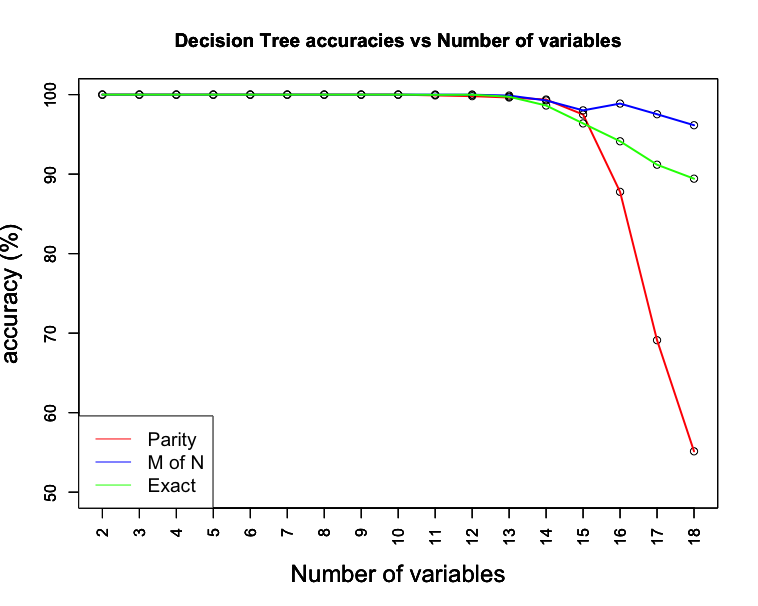
\includegraphics[width = 1 \linewidth]{Figures/DTone.png}
        \caption{Decision tree accuracies}
        \label{fig:DTvsNN_DT}
    \end{subfigure}%
    
    
    \begin{subfigure}[t]{0.4\textwidth}
        \centering
        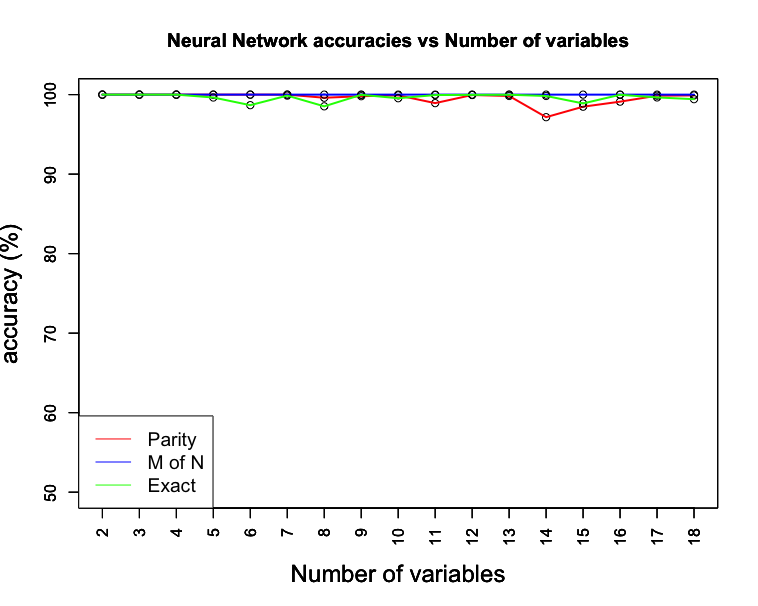
\includegraphics[width = 1 \linewidth]{Figures/NNone.png}
        \caption{Neural network accuracies}
        \label{fig:DTvsNN_NN}
    \end{subfigure}% 
    \caption{The accuracies of the decision tree (A) and neural network (B) on the parity condition (red), M-out-of-N condition (blue) and exact value condition (green) for varying number of variables.}
    \label{fig:DTvsNN}
\end{figure}

Additionally, in order to investigate how well the systems perform with noise, a particular percentage of the instances of the training dataset are given a ``noisy variable''. These noisy variables have their values inverted, such that a 1 becomes a 0 and a 0 becomes a 1. It should be noted that inverting the value of a variable does not always mean that the outcome becomes incorrect. Varying the percentage of instances with a noisy variable between 0 and 100\% yields the graphs shown in Figure \ref{fig:SBF_noise}. These graphs display the mean accuracies of the decision tree (red) and the neural network (blue) on the specific test set for each of the three symmetrical Boolean functions.  The accuracies are average accuracies across values of $n$ ranging from 2 to 10 and across all possible values of $m$.


  \begin{figure}[p]
    \centering
   \begin{subfigure}[t]{0.4\textwidth}
        \centering
        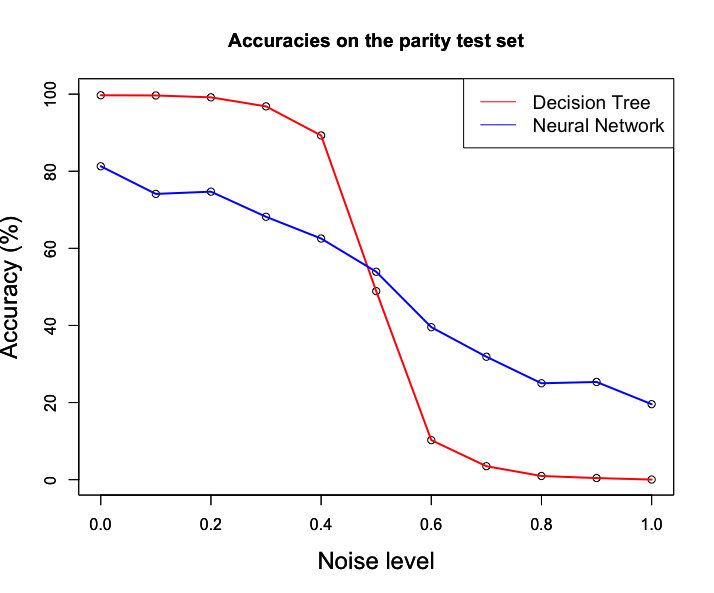
\includegraphics[width = 1 \linewidth]{Figures/SBF_PU.png}
        \caption{}
        \label{fig:SBF_PU}
    \end{subfigure}%

    \begin{subfigure}[t]{0.4\textwidth}
        \centering
        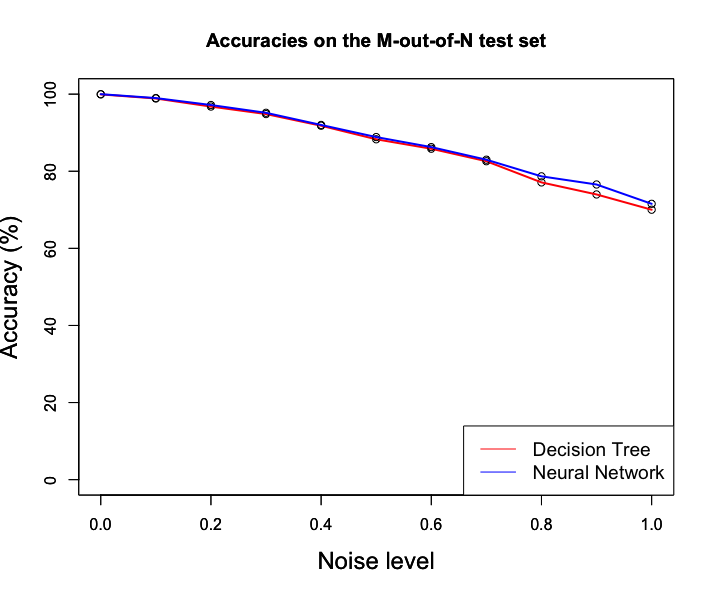
\includegraphics[width = 1 \linewidth]{Figures/SBF_MU.png}
        \caption{}
        \label{fig:SBF_MU}
    \end{subfigure}%

    \begin{subfigure}[t]{0.4\textwidth}
        \centering
        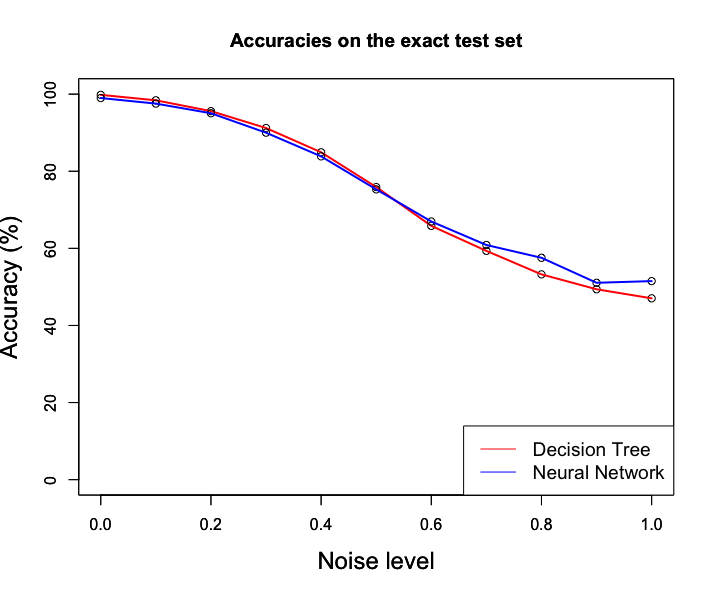
\includegraphics[width = 1 \linewidth]{Figures/SBF_EU.png}
        \caption{}
        \label{fig:SBF_EU}
    \end{subfigure}%
    \caption{The effect of varying levels of noise on the accuracies of the decision tree algorithm (red) and the neural network (blue) after training on the parity function (a), the M-out-of-N function (b) and the Exact value function (c).}
    \label{fig:SBF_noise}
\end{figure}

Even under extreme levels of noise, the systems are still able to learn the M-out-of-N and exact value function quite effectively, showing the robustness of machine learning results. The parity function is a special case, as its output is dependent on whether the amount of 1's in the input vector is odd or even. This means that if an instance in the training dataset has a noisy variable, that instance automatically has the wrong output. If all of the instances in the training set have a noisy variable, the systems simply learn that an even number of 1's should yield true, which is the complete opposite of the parity function.%%%BV WHAT DO YOU WANT TO SAY HERE? CONNECTION TO DATA SHOWN?

\subsection{Multiple Condition Datasets}
As mentioned earlier, systems that are able to learn how to solve a combined problem, may not necessarily have learned all of the conditions that make up the combined problems; there can be an interaction effect between the conditions. To investigate this, neural networks and decision trees were trained and tested on datasets that include two of the three symmetrical Boolean functions. First of all, the interaction between the parity function and the exact value function is examined, followed by the interaction between the parity function and the M-out-of-N function, and lastly the interaction between the M-out-of-N function and the exact function will be explored. For all three combinations, the number of variables per function will be varied between 2 and 10, thus creating instances with 4 to 20 variables when combining the two conditions.  Just as in the results of the single conditions, the accuracies of the M-out-of-N function and the exact function are averaged over all possible values of $m$. For each interaction, three accuracies will be examined per system: the accuracy on the general test set, the accuracy on a specific test set of the first condition and a specific test set of the second condition.

\begin{table}[h!]
\centering
\caption{The mean accuracies of the decision tree on each test set after training on each interaction.}
\resizebox{\columnwidth}{!}{%
\begin{tabular}{|c|c|c|c|}
\hline 
 & General &  Function 1 & Function 2 \\ 
 & accuracy &  accuracy & accuracy \\ 
\hline 
Parity, Exact &  98.50 & 17.48 & 78.75 \\ 
\hline 
Parity, M-out-of-N  & 99.99 & 30.36 & 81.75 \\ 
\hline 
M-out-of-N, Exact & 99.99 & 96.00 & 32.53 \\ 
\hline 
\end{tabular} %
}
\label{tbl:interactions_DT}
\end{table}

\begin{table}[h!]
\centering
\caption{The mean accuracies of the neural network on each test set after training on each interaction. }
\resizebox{\columnwidth}{!}{%
\begin{tabular}{|c|c|c|c|}
\hline 
 & General &  Function 1 & Function 2 \\ 
 & accuracy &  accuracy & accuracy \\ 
\hline 
Parity, Exact & 99.65 & 14.59 & 78.31 \\ 
\hline 
Parity, M-out-of-N & 100.00 & 30.59 & 81.65 \\ 
\hline 
M-out-of-N, Exact & 99.99 & 99.88 & 26.14  \\ 
\hline 
\end{tabular}%
} 
\label{tbl:interactions_NN}
\end{table}

An overview of the average accuracies of the decision trees and neural networks is given in Table \ref{tbl:interactions_DT} and Table \ref{tbl:interactions_NN} respectively. These show the mean accuracies for each interaction on each of the different test sets: the general test set, and one test specific test set for each of the two functions of the interaction. What is clear from these tables, is that the mean accuracy of both the neural network and the decision tree on the general test set is quite high for each interaction. However, the accuracies on the specific test sets, which indicate how well the functions themselves are learned, are almost always a lot lower. With the parity-exact interaction, for instance, the decision tree algorithm preforms with an accuracy of 98.5\% on the general test set, but only 17.5\% on the parity test set and 78.8\% on the exact test set. This is shows that a system can perform with a high accuracy, even if it has not learned all of the conditions correctly. The accuracies of the neural network and the decision tree system are also quite similar to each other, which shows that the trends in accuracies are not limited to a single machine learning algorithm. The relationships between the number of variables for each function and the accuracies of each of the tests sets are recorded as well, an example of which can be seen in the heatmaps of Figure \ref{fig:Heatmap_ME}. These display the mean accuracies of the decision tree on the three different test sets for the M-out-of-n and exact value function interaction versus the number of variables of both functions on the x- and y-axis.

 \begin{figure}
    \centering
    \begin{subfigure}[t]{0.45\textwidth}
        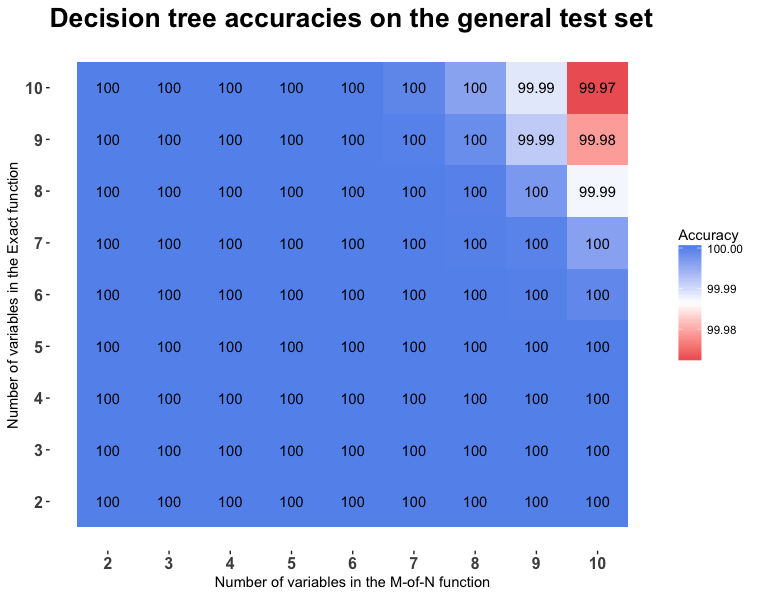
\includegraphics[width = 1 \linewidth]{Figures/Heatmap_ME_DT_general.png}
		\caption{}       
        \label{fig:Heatmap_ME_DT_general}
    \end{subfigure}%

    \begin{subfigure}[t]{0.45\textwidth}
        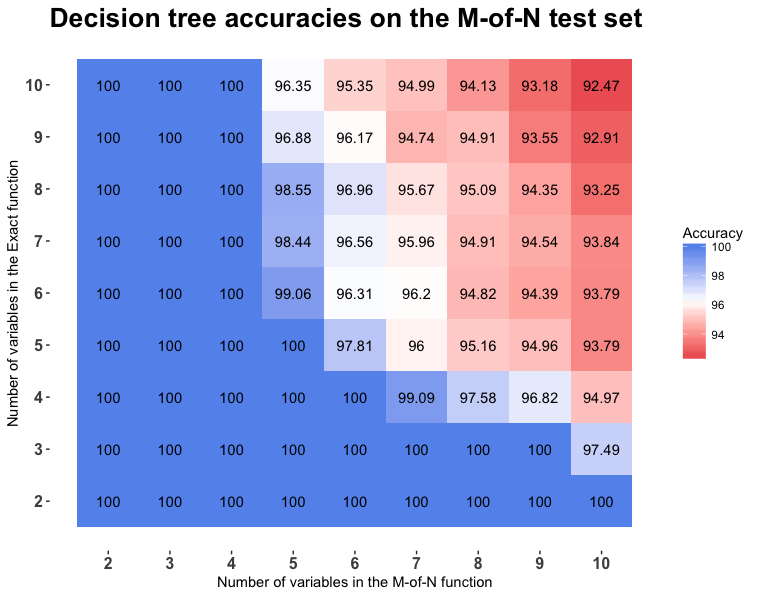
\includegraphics[width = 1 \linewidth]{Figures/Heatmap_ME_DT_M.png}
		\caption{}       
        \label{fig:Heatmap_ME_DT_M}
    \end{subfigure}% 

   \begin{subfigure}[t]{0.45\textwidth}
        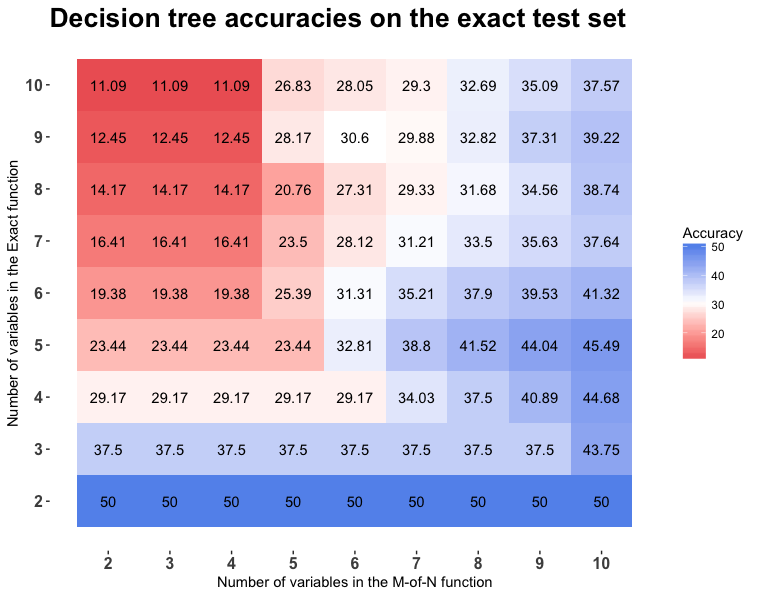
\includegraphics[width = 1 \linewidth]{Figures/Heatmap_ME_DT_E.png}
		\caption{}       
        \label{fig:Heatmap_ME_DT_E}
    \end{subfigure}% 
    \caption{The mean accuracies of the decision tree system on the different test sets after training on the training set with a M-of-N function (x-axis) and an exact function (y-axis) with varying numbers of variables in each function.}
    \label{fig:Heatmap_ME}
\end{figure}

The accuracies on the general test set (Figure \ref{fig:Heatmap_ME_DT_general}) show the overall performance of the decision tree system on the combined problem. Unsurprisingly, more M-out-of-N and exact value function variables lead to a decrease in accuracy; as the problem becomes more complex, it is more difficult for the system to learn. Figure \ref{fig:Heatmap_ME_DT_M} displays how well the M-out-of-N function is learned by the system, and a similar decrease in accuracy can be observed when more variables are used in the data. Interestingly, the number of M-out-of-N variables has a bigger influence on the accuracy on this test set than the number of exact value variables. This could be because functions with more variables are more difficult for the systems to learn. In Figure \ref{fig:Heatmap_ME_DT_E}, which displays how well the exact value function is learned, a different effect can be observed. The accuracy on this test set decreases with more exact value variables, but increases with more M-out-of-N variables. So a larger number of
exact value variables decreases how well the M-out-of-N function is learned, while a larger number of M-out-of-N variables increases how well the exact function is learned. 

We have investigated these effects for all combinations of the conditions. A summarized overview of the effects that the conditions have in the other interactions is shown in Table \ref{tbl:highlow}. 

\begin{table}[h!]
\centering
\caption{This table shows the  effect that a high number of variables of a function has on the performance of a system (in terms of learning the function) for all functions that it interacts with.}
\resizebox{\columnwidth}{!}{%
\begin{tabular}{|c|c|c|c|}
\hline 
Performance on $\downarrow$ & Parity & Exact & M-out-of-N \\ 
\hline 
Parity & - & decreases & decreases \\ 
\hline 
Exact & increases & - & decreases \\ 
\hline 
M-out-of-N & increases & decreases & - \\ 
\hline 
\end{tabular}%
}
\label{tbl:highlow}
\end{table}


\section{Discussion}
Our findings show that in our generalized setting with symmetric Boolean functions a high performance in terms of classification accuracy does not guarantee that the system has learned the conditions that define the dataset, as evident by Table \ref{tbl:interactions_DT} and Table \ref{tbl:interactions_NN}. Also we saw that when dealing with interactions, the number of variables of a function can either increase or decrease how well a system learns the function, depending on the other function that is in the dataset. The accuracy on the parity test set increases with a low number of parity variables in both the interaction with the exact value function and the M-out-of-N function. The accuracy on the exact value test set increases with a high number of exact variables in the interaction with the parity function and with a low number of exact variables in the interaction with the M-out-of-N function. Similarly, the accuracy on the M-out-of-N test set increases with a high number of M-out-of-N variables in the interaction with the parity function, and with a low number of M-out-of-N variables in the interaction with the exact value function. Table \ref{tbl:highlow}  shows that higher numbers of parity variables always have a negative effect on the how well the parity function is learned, regardless of other the functions that define the dataset. This is also true for the other two functions, except when interacting with the parity function; when interacting with the parity function, a high number of exact/M-out-of-N variables has a positive effect. Earlier results %%%%BV REFERENCE?
already showed that the parity function is more difficult to learn than the other two functions. This, combined with the finding of Table \ref{tbl:highlow} suggests that the interference of the parity function has a greater negative impact on how well the the exact and M-out-of-N function are learned than the number of variables of said function. This could explain why the increase in variables creates a increase in learning the exact and M-out-of-N functions in combination with the parity function. 

The experiment with the symmetrical Boolean functions has confirmed that the neural network and the decision tree algorithm can learn the XOR condition and its generalized form, the parity function, if there is no interference from other variables. Compared to the M-out-of-N and exact value function, the parity function seems to be the most difficult function for the machine learning systems to learn. Both neural networks and decision trees, however, can learn them with sufficient training. Once multiple conditions are presented to the systems at the same time, however, the systems are unable to learn the conditions as well. The accuracies on the general test sets are still quite high for all possible interactions between the functions, but the systems do not learn the functions themselves as well. This supports the claim that a high classification accuracy is no guarantee that the right rationale is used in the classification process. The accuracies on the general test set and on each of the functions individually can be seen in Table \ref{tbl:interactions_DT} and Table \ref{tbl:interactions_NN}. It is interesting to see how systems can perform with an accuracy of almost 100\% on the general test set, yet fail dramatically on the test sets of the individual functions. This indicates that they do not actually learn these functions, but rather a different function that somehow accurately maps the input to the output. There must therefore be a confounding structure within the data that the systems learn instead of the original, intended structure. 

In most of the experiments, the performances of the neural network and the decision trees were quite similar. When considering the fact that decision trees are transparent and much more easy to comprehend, they would appear to be superior to the ``black box''  neural network. However, the experiments in this study used relatively simple functions and conditions, which both connectionist and symbolic machine learning techniques can learn. %When dealing with image or speech data, for instance, the (deep) neural networks will generally outperform the symbolic learning techniques. This is because neural networks are better at generalizing, whereas decision trees attempt to map out the entire training set. Due to these inherent differences, they are generally used for different purposes. 

\section{Conclusion}
\noindent In the future, machine learning algorithms that simply execute a task with a high performance will not suffice; an explanation of their decision making will be required \cite{gunning2017explainable}. This explanation, however, is dependent on the reasoning of the systems; if the reasoning is unsound, the explanation will be unsound as well. This study has shown that machine learning algorithms do not always internalize the structure of their training data as we would expect. With regards to the emerging XAI techniques and the explainable models that they generate, the unsound rationales of machine learning systems can form a hindrance in creating an understandable explanation. 

%%%BV CHECK REFERENCES (see also bibtex warnings)
%%%BV PLACE OF FIGURES AND TABLES (liever aan uiteinden van kolommen; top of bottom)

\bibliography{references}
\bibliographystyle{aaai}
\end{document}
